\begin{frame}
    \frametitle{Terminology}
    \framesubtitle{Generative Adversarial Networks(GAN)}
    \begin{figure}
        \centering
        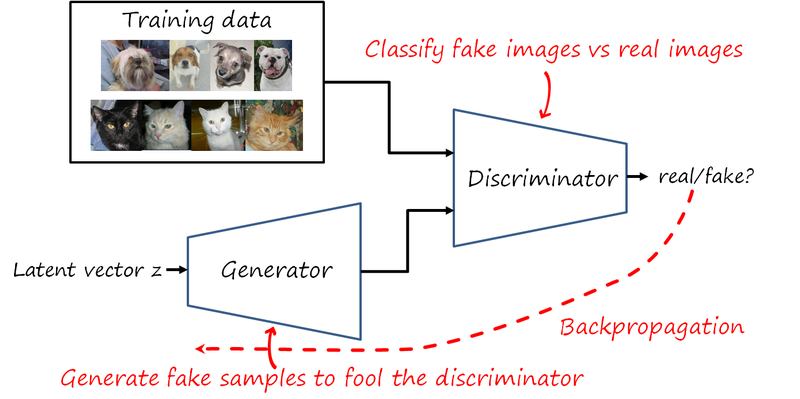
\includegraphics[width=0.65\linewidth]{images/blog_gan.png}
        \caption{GAN training process}
    \end{figure}
    \tiny{\footnotemark \url{http://www.lherranz.org/2018/08/07/imagetranslation/}}
\end{frame}
\note{
    \begin{itemize}
        \item Generative Adversarial Networks: Zwei Netzwerke, Generator und Diskriminator, die gegeneinander trainiert werden        
            \begin{itemize}
                \scriptsize\item Generator: versucht die verteilung der Trainingsdaten zu lernen ohne diese zu kennen
                \scriptsize\item Diskriminator: Unterscheidet zwischen echten und generierten Bildern        
            \end{itemize}            
        \item Loss Function: Min-Max Game zwischen Generator und Diskriminator 
    \end{itemize}
}

\begin{frame}
    \frametitle{Terminology}
    \framesubtitle{Generative Adversarial Networks(GAN) - Loss Function}
    \begin{block}{GAN Loss Function}
        
        \begin{equation}
            \min_G \max_D \mathcal{L}(D,G) = \mathbb{E}_{x \sim p_{\text{data}}(x)}[\log D(x)] + \mathbb{E}_{z \sim p_z(z)}[\log(1 - D(G(z)))]
        \end{equation}
    
    \end{block}
    \tiny{\footnotemark \url{http://www.lherranz.org/2018/08/07/imagetranslation/}}
\end{frame}
\note{           
    \begin{itemize}
        \item x: echtes bild
        \item z: Zufälliger Input für den Generator
        \item $p_{\text{data}}(x)$: Wahrscheinlichkeitsverteilung der echten Daten
        \item $p_z(z)$: Wahrscheinlichkeitsverteilung des zufälligen Inputs
        \item $D(x)$: Wahrscheinlichkeit, dass x ein echtes Bild ist
        \item $G(z)$: Generiertes Bild                        
    \end{itemize}
    Diskriminator wird trainiert um die Wahrscheinlichket, dass korrekte Label zu erkennen zu maximieren.\\
    
    Probleme: Früh im Training ist der Generator noch sehr schlecht, deswegen wird der $log(1 - D(G(z)))$ Term sehr groß und der Gradient verschwindet.\\
    In Praxis wird $logD(G(z))$ verwendet, um dieses Problem zu umgehen.\\ 
    
    Weiterentwicklungen: DCGANs, Wasserstein Distance als Loss Function oder PG-GANs nur Name dropping

}
    
% ---------- CycleGAN ----------
\begin{frame}
    \frametitle{Terminology}
    \framesubtitle{CycleGAN}
    \begin{figure}
        \centering
        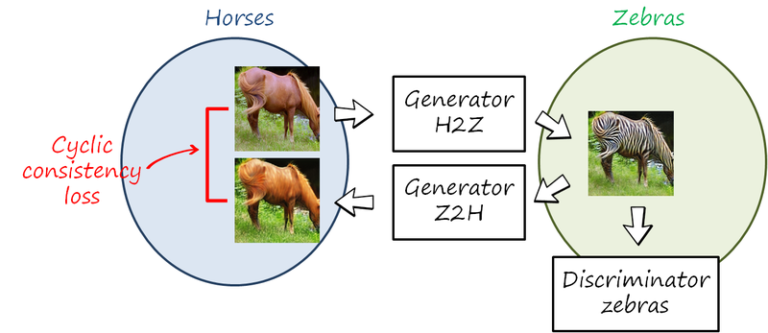
\includegraphics[width=0.78\linewidth]{images/blog_cyclegan_h2z2h-768x333.png}
        \caption{CycleGAN Architecture}
    \end{figure}
    \tiny{\footnotemark \url{http://www.lherranz.org/2018/08/07/imagetranslation/}}
\end{frame}
\note{
    \begin{itemize}    
        \item Zwei GAN Netzwerke mit jeweils eigenen Generator und Diskriminator
        \item Ein Netzwerk generiert Bilder von Domain X zu Domain Y und das andere Netzwerk generiert Bilder von Domain Y zu Domain X
        \item Ein Cycle Konsistenz Loss wird verwendet um sicherzustellen, dass das generierte Bild nach der Transformation wieder zum Originalbild zurückgeführt werden kann
    \end{itemize}
}

\begin{frame}
    \frametitle{Terminology}
    \framesubtitle{CycleGAN - Loss Function}
    \begin{block}{CycleGAN Loss Function}        
        \begin{equation}
            \mathcal{L}_{\text{cycle}}(G, F) = \mathbb{E}_{x \sim p_{\text{data}}(x)} [\lVert F(G(x)) - x \rVert_1] + \mathbb{E}_{y \sim p_{\text{data}}(y)} [\lVert G(F(y)) - y \rVert_1]
        \end{equation}
    \end{block}
    \tiny{\footnotemark \url{http://www.lherranz.org/2018/08/07/imagetranslation/}}
\end{frame}
\note{
    \begin{itemize}
        \item $G(x)$: Generiertes Bild von Domain X zu Domain Y
        \item $F(y)$: Generiertes Bild von Domain Y zu Domain X
        \item $F(G(x))$: Generiertes Bild von Domain X zu Domain Y und zurück zu Domain X
        \item $G(F(y))$: Generiertes Bild von Domain Y zu Domain X und zurück zu Domain Y
        \item $L_1$ Loss wird verwendet, um die Differenz zwischen dem generierten Bild und dem Originalbild zu berechnen
    \end{itemize}
}
    
    
        
% ---------- UNet and Skip Connections ----------
\begin{frame}
    \frametitle{Terminology}
    \framesubtitle{UNet and Skip Connections}
    \begin{figure}
        \centering
        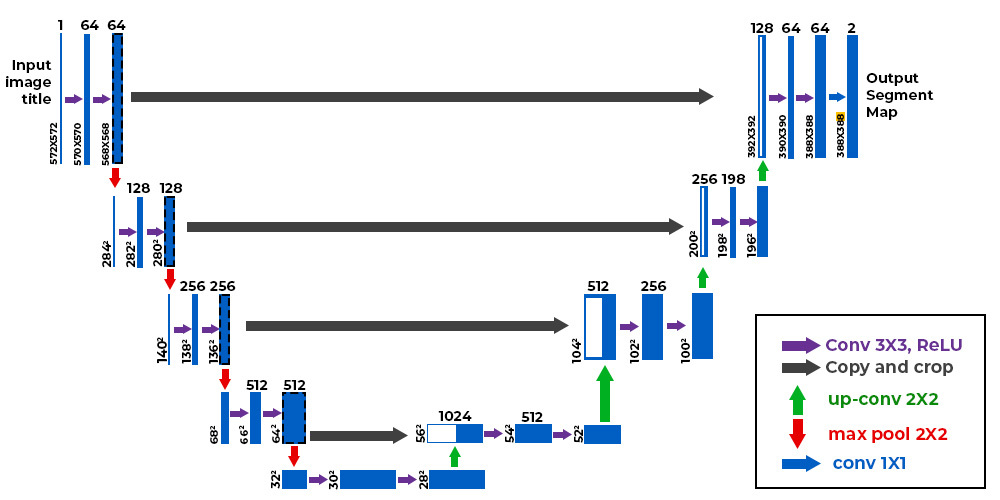
\includegraphics[width=0.6\linewidth]{images/Group14.jpg}
        \caption{Architecture}
    \end{figure}
\end{frame}
\note{
    \begin{itemize}
        \item UNet: Architekture wurde erstmals 2015 vorgestellt von im Paper U-NET: Convolutional Networks for Biomedical Image Segmentation von Olaf Ronneberger, Phillip Fischer und Thomas Brox von der Uni Freiburg
        \item Architektur gewann 2015 den ISBI Cell Tracking Challenge mit großem Vorsprung
        \item Encoder Pfad: Mehrere Blöcke von convolutional layers mit ReLU activation und max pooling. Reduziert die Dimensionalität des Inputs
        \item Decoder Pfad: Mehrere Blöcke von convolutional layers mit RelU activation und upconvolution. Erhöht die Dimensionalität des Inputs. Außerdem Concatenation mit entsprechenden Encoder Pfad
        \item Skip Connections: Verbindung zwischen Encoder und Decoder Pfad. Hilft details zu erhalten, die im Encoder verloren gehen würden
    
    \end{itemize}
}
    
% ---------- LoRA Weights ----------
\begin{frame}
    \frametitle{Terminology}
    \framesubtitle{LoRA Weights}
    \begin{figure}
        \centering
        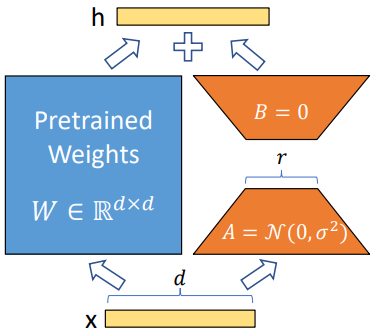
\includegraphics[width=0.4\linewidth]{images/Bildschirmfoto vom 2024-04-15 10-21-59.png}
        \caption{\textbf{Lo}w \textbf{R}ank \textbf{A}daption}
    \end{figure}
    \tiny{\footnotemark \url{https://arxiv.org/pdf/2106.09685}}

\end{frame}
\note{
    \begin{itemize}
        \item LoRA wird zum fine tunen von vortrainierten Modellen verwendet
        \item LoRA beruht auf der Idee, dass die Gewichtsmatrix eines Modells einen niedrigen Rang hat, was bedeuten würde dass der großteil von Informationen in einigen wenigen Dimensionen ausgedrückt werden kann
        \item Bei Model finetuning ohne LoRA würde man das orginale gewicht fixieren und ein neus gewicht $\delta W$ lernen, die neue Gewichtsmatrix hier h im Bild wäre dann orginales Gewicht + $\delta W$
        \item Hier setzt LoRA an, es wird angenommen, dass die neue Gewichtsmatrix einen niedrigen Rang hat und kann dann als Produkt von zwei niedrig rangigen hier r Matrizen dargestellt werden
        \item A ist zu Beginn Guaß-verteilt, B zu 0
        \item mit Adam wird dann der Rang von A und B optimiert
        \item Im Paper wurde gezeigt, dass für GPT-3 175B ein rang von 1 oder 2 ausraucht, obwohl die Rang der Gewichtsmatrix 12,288 beträgt
    \end{itemize}
}

% ---------- Paired vs unpaired data ----------
\begin{frame}
\frametitle{Terminology}
\framesubtitle{Paired vs unpaired data}
\begin{columns}
    \column{0.5\textwidth}
    \centering    
    \begin{figure}
        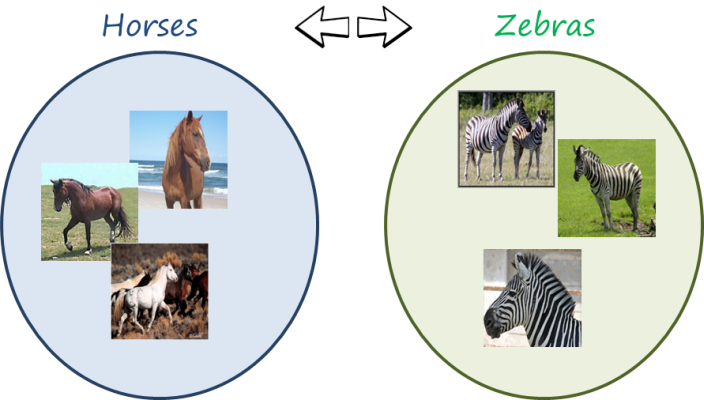
\includegraphics[width=0.75\textwidth]{images/blog_unpairedimagetranslation2.png}
        \caption{Unpaired Data}
    \end{figure}

    \column{0.5\textwidth}    
    \centering    
    \begin{figure}        
        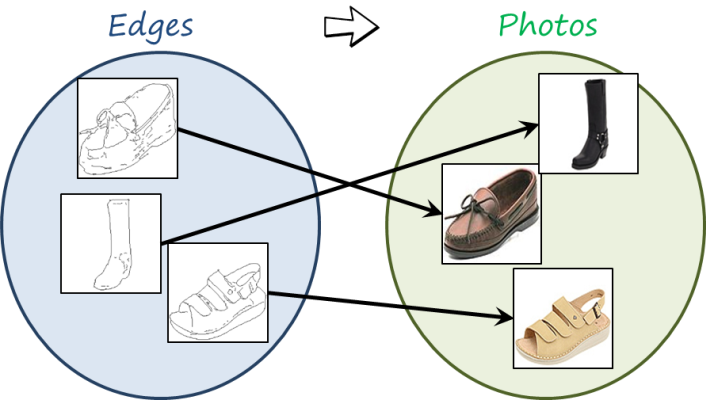
\includegraphics[width=0.75\textwidth]{images/blog_pairedimagetranslation.png}
        \caption{Paired Data}
    \end{figure}
    \end{columns}
\end{frame}
\note{
    \begin{itemize}
        \item Paired data: Jedes Bild in Domain X hat ein korrespondierendes Bild in Domain Y. Z.b Hier Bild von Schuhen und ein Bild von Kanten von Schuhen
        \item Unpaired data: Paired data ist für viele Anwendungen nicht verfügbar. z.B wie im Paper Pferde zu Zebras, Tagbild zu Nachtbild, Nachtbild zu Tag, etc.
        \item In dem Paper wird eine Architektur vorgestellt, die einmal mit paired und einmal mit unpaired Daten trainiert wird
        \item Paired Model heißt CycleGAN-Turbo
        \item Unpaired Model heißt Pix2Pix-Turbo
    \end{itemize}

}
